\chapter{Conclusion} \label{chap:conclusion} \minitoc

\section{Hypothesis Revisited}

In Section \ref{sec:hypothesis} we defined our hypothesis or main question to address as whether sliding window aggregations and outlier detection methods combined could be used to detect data pattern shifts in data streaming scenarios in the presence of high volumes of high velocity, highly skewed and seasonal data in real-time and with a low memory footprint. Before discussing our hypothesis, we revisit the research questions posed in Section \ref{sec:rqs} and provide answers to them. 

\subsubsection*{(RQ1) What aggregation can we use to properly encode data distributions?}
First, we searched for a set of aggregations that would encode our distribution in the best way. Later on, we concluded that a simple histogram is better than any other set of aggregations. Histograms are a representation of the distribution of numerical data thus being ideal to encode the distribution of feature values. 

In brief, the answer to RQ1 is that we can use histogram aggregations to properly encode data distributions.

\subsubsection*{(RQ2) How can we maintain such an aggregation in a sliding window fashion in real-time with constant memory usage?}

This research question really is about two things: maintaining the sliding window aggregation in real-time and keeping its memory usage constant.

The aggregation in question is an histogram aggregation.
An histogram requires storing a fixed-size list of bins and corresponding counts, regardless of the volume of data. This means that for ever growing volumes of data our memory consumption stays the same.

However, maintaining a sliding window histogram in real-time is an harder challenge. Traditionally, sliding window maintenance requires evicting the oldest element from the window when a new one is inserted and updating the aggregation state. We could maintain the histogram in constant time using a Subtract-On-Evict (SOE) algorithm (Algorithm \ref{pseudo:soe}): for each new event, we would evict the oldest one and decrement the bin it belonged to and insert the new event in the window while incrementing the bin it belongs to. However, using this approach, we violate our sublinear memory consumption, because now we have to keep the entire window contents in memory, hence we grow linearly regarding sliding window size. We instead propose an EMA-like approximate histogram aggregation, in Section \ref{sec:ema-hist}. An EMA-like histogram has constant memory complexity and can be maintained in real-time.

To summarize, EMA-like approximate histogram aggregations, defined in Section \ref{sec:ema-hist}, have constant memory and time complexity and can be maintained in a sliding window fashion.

\subsubsection*{(RQ3) How can we measure divergence between the reference and sliding window aggregations?}
Statistical tests that measure the similarity between two probability distributions are common in the literature. Tests like Kolmogorov–Smirnov, Wassertein or Jensen–Shannon (the one we used) provide a bounded measure of distance between two probability distributions, or histograms. 

In brief, since the aggregation we use is an histogram, we can use statistical tests that measure similarity between probability distributions. We chose to use the Jensen–Shannon Divergence (JSD). The JSD takes as input two histograms and outputs a value between 0 and 1. The closer this value is to 0 the more similar the distributions are. On the other hand, a JSD value of 1 represents two different distributions. We chose to use the JSD metric due to its simplicity and leave as future work the usage of other statistical tests.


\subsubsection*{(RQ4) Based on a divergence measure, when should we raise an alert?}
Statistical divergence tests provide fixed bounds for the measurement value. In the case of the Jensen–Shannon Divergence (JSD), the output ranges from 0 to 1. This research question poses the following challenge: how can we threshold a JSD value? In other words, do we alert a feature as divergent if the JSD measure is above 0.6? Or if above 0.99? How can we threshold this value?

In Section \ref{sec:sampling-batch}, we explain how we define the threshold and hence define when we raise an alert. In our batch phase, we make a number of samples and measure the JSD distance between the histogram aggregations of those samples and our reference histogram aggregation. We end up with a list of JSD values. Given a new JSD value, we check against the now known distribution of JSD values and alert if above a certain percentile. Note that defining a threshold percentile is easier, because we are defining a probability: alerting above the 99th percentile means alerting for hypothesis with 1\% probability.

In brief, we build the distribution of divergence values in batch and use it to compare a future divergence value and find out its probability. If said divergence value has a very low probability (\textit{e.g.}, 1\% or less), then we raise an alert.

\subsubsection*{Hypothesis Discussion}
In our synthetic data experiments, we were able to detect all of the introduced anomalies. Additionally, we were able to do it achieving very high streaming throughputs. In the real data experiments, once again, we managed to achieve high troughputs but the produced alerts were not very accurate. We defer further investigation to future work because of the time constraints of this thesis but leave open the possiblity that the approximate aggregation value is more inaccurate than what we thought it would be, due to the fact that the EMA tail holds all past events.

Overall, our set of tests supports the claim that sliding window aggregations and outlier detection methods can indeed be combined to detect data pattern shifts in streaming scenarios, with constant time and memory complexity.

\section{Contributions}
We summarize our contributions as follows:

\begin{enumerate}
    \item a two-phased and two-windowed univariate subsequence outlier detection method, classified according to the taxonomy in Section \ref{sec:uni-sub-out} and detailed in Chapter \ref{chap:my-work}, that is lightweight and works for real-time stream monitoring
    
    \item an histogram aggregation based on Exponential Moving Averages, that replaces the entire sliding window contents by a lighter representation, resulting in a constant in time and space complexity sliding window aggregation
    
    \item a set of synthetic datasets and experiments where the method in question accurately detected anomalies
    
    \item experiments on real data that showed unexpected results but where we provide insights and possible hypothesis to test for future work
\end{enumerate}

\section{Future Work}

First and foremost, we believe the next steps are to reason about the obtained results in the real data experiments and find the root cause for the existence of many and large alert periods. As possible hypothesis to test, we suggest testing with EMAs with higher smoothing factors, so that past events are forgotten faster; additionally, we suggest decreasing $\gamma$, which further increases the number of samples to make in the batch phase.

In this thesis we used the Jensen–Shannon Divergence (JSD) as statistical test to measure the distance or divergence between our reference and target sliding window aggregation. We chose to use the JSD metric due to its simplicity and because it was used in previous work successfully \cite{SAMM}. We believe that future work comprises testing new distances in the literature. In particular, we believe the Wassertein distance is worth trying next, and illustrate why in Figure \ref{fig:wasserteinvsjsd}.
\begin{figure}[!htb]
    \begin{center}
      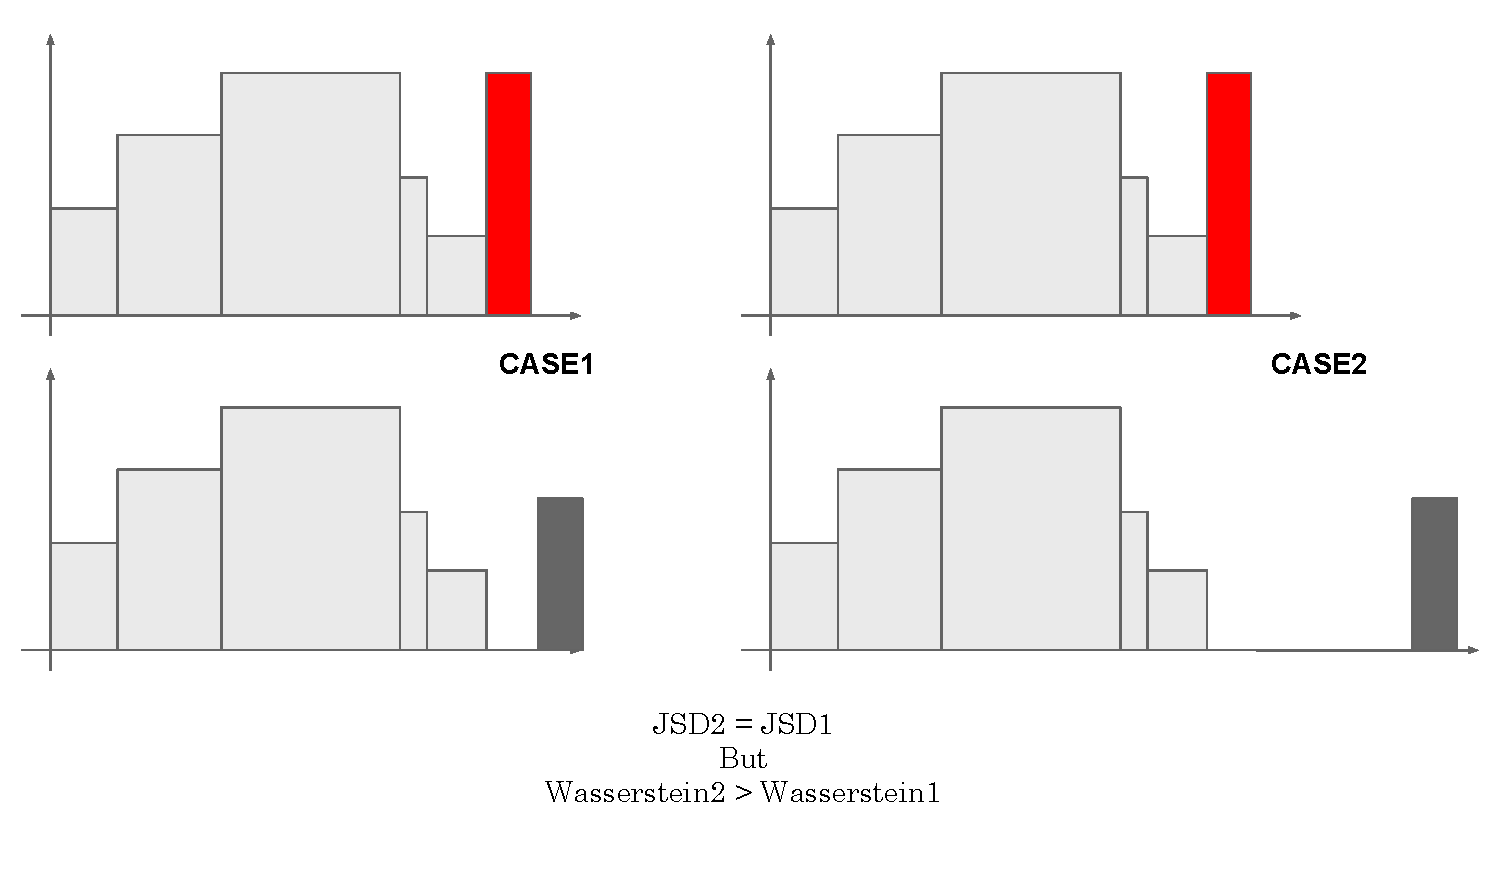
\includegraphics[scale=0.6]{figures/wasserstein-vs-jsd.pdf}
      \caption{Wassertein vs Jensen–Shannon distances}
      \label{fig:wasserteinvsjsd}
    \end{center}
\end{figure}
The Wassertein distance measures the work required to transport the probability mass from one histogram to the other. This measure will be larger the further way the probability mass is. In Figure \ref{fig:wasserteinvsjsd} scenario, while in the JSD measure is the same for both cases, the Wassertein distance is larger in case 2 because the probability mass has to be transported further.

In this thesis we had to deal with the multiple test problem and apply a multiple test correction. In our case, we used Holm-Bonferroni due to its simplicity and because it controls the family wise error rate with a larger power than some other methods (thus providing a good trade-off between simplicity and power). There are many other multiple test correction methods, and we leave the testing of each as future work.

Lastly, we propose another type of validation method. We mentioned in the beginning that our objective is to detect data pattern shifts before the performance of the systems relying on the data declines. We propose a test where we train a Machine Learning model on a reference period and measure its prediction accuracy on a target period. Then, we propose running our method on reference and target periods to find out timestamps with a high number of divergent features. We propose that the model is retrained at these timestamps (tantamount to system reconfiguration) and then used to predict for the remaining target period. Finally, we propose that the accuracy should be compared to the previously observed model performance, expecting it to be better after retraining in one of the high divergent timestamps.
